\chapter{系统功能需求分析与系统架构设计}

\section{系统功能需求}
文献X中表明,在一确定的CNN中,卷积的计算时间占据了至少85\%,因此若想制作一款CNN加速器,那么急需解决的问题就是如何加速图像的卷积计算。
卷积计算虽然参数相比于CNN中全连接层少,但其计算量非常大,而且通常为简单的乘加操作。
    \subsection{传统架构}
        \subsubsection{CPU}
        首先,CPU在深度学习计算中很重要,例如使用了16000颗CPU搭建的“Google Brain”网络,又比如1920颗CPU搭建的“AlphaGo”。如今,CPU依旧是主流深度学习平台的重要组成部分,
        但在深度学习领域,CPU在架构方面有着先天的不足,从芯片面积上看,Cache和Control单元占据了绝大部分面积,而用于计算的ALU面积却比较少;每颗核心都狠强大,但核心数量少。
        因此CPU重在数据调度,并不擅长大规模简单的运算。
        \subsubsection{GPU}
        反观GPU,虽然每颗核心都比较弱,只能完成简单的计算,但通常一个GPU都是上百上千个核心,芯片面积上用于计算的ALU单元占据了绝大部分,当所有核心都被调用起来,其运算能力远远大于CPU。
        同时,GPU普遍采用DDR5片上显存颗粒,更高的工作频率带来了更快的数据读写速度,而且总线带宽大。
    \subsection{异构的优势}
        目前做深度学习开发普遍采用CPU+GPU这种异构形式作为首要开发平台,既可以利用CPU强大的调度能力也可以利用GPU超快的计算速度,但这种模式是一种通用级的解决方法,应用在细分的专业领域边显的过于臃肿,不仅设备体积大,功耗也高。
        一般情况下,当模型训练完成后,需要利用模型进行推理计算,这部分不需要复杂的反向传播计算,若继续采用训练时的CPU+GPU平台,不仅造成资源浪费,量产时成本极高。
        因此针对推断,我们希望能找到一种低功耗、高性能的解决方案,因此使用FPGA和ASIC具有极大的优势。

        相比于通用的CPU+GPU的架构,CPU+FPGA/ASIC组成的异构平台具有更高的计算能效比,同时成本更低,十分适合当下嵌入式IoT领域对低功耗、高灵活性的需求。
        相比于受限于冯诺依曼架构的CPU/GPU,FPGA和ASIC在设计时可以通过多核心、流水线等技术充分发挥并行计算的特性,大大提高数据吞吐量。

\section{系统架构设计}
    针对本章第一节的需求,本文通过调研当前硬件加速方案,参考论文X的思想设计了一套针对CNN计算加速的方案。
    \begin{figure}[h]
        \centering
        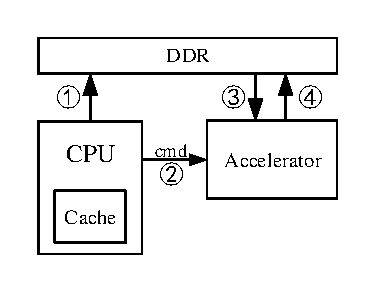
\includegraphics{../pdf/system.pdf}
        \caption{CNN加速系统架构示意图}
        \label{}
    \end{figure}

\section{开发环境}
    \subsection{HLS}
    HLS(High Level Synthesis)也既高层次综合技术,是Xilinx公司大力推广的一项FPGA开发技术。该技术使用C/C++作为开发语言,可以充分利用该语言中提供的数据结构进行FPGA开发。
    最终可以生成Verilog或VHDL语言。

    通过HLS使得软件工程师可以不用了解FPGA和Verilog,也可以使用FPGA进行硬件加速,大幅减少FPGA开发难度和开发周期。该技术已应用在SDAccel、SDSoC等软件中,目前在偏算法的视频图像处理领域有着广泛的应用。

    但简单易用的东西背后都会带来不必要的性能浪费。与传统HDL开发相比,HLS无法对电路进行精细化操作,因此虽然HLS能够大大缩短开发周期,但从能性能方面传统HDL开发更具有优势。
    \subsection{OpenCL}
    HLS可以进行算法的快速实现,但是并不适合大规模系统开发。OpenCL的出现给人们带来使用高层次综合进行大规模系统开发的希望。
    OpenCL(Open Computing Language)即开放运算语言,是第一个面向异构系统通用目的并行编程的开放式、免费标准,也是一个统一的编程环境,广泛使用于CPU,GPU,DSP,FPGA等并行处理器的开发。
    其提供了一系统采用C/C++封装的API,编写的程序可以在支持OpenCL的设备上运行。
    与HLS相似,OpenCL也使开发人员脱离底层电路,允许在系统层面进行开发。由于OpenCL是跨平台的,因此可以很容易的将原来CPU或GPU的代码做些许改动就能在支持OpenCL的FPGA上运行。
    \subsection{敏捷型开发}
    敏捷型开发思想源于软件工程,其宗旨是以用户需求进化为核心,采用迭代、循序渐进的方法进行软件开发,在此过程中软件一直处于可工作状态。软件之所以可以采用敏捷型开发是因为其反馈环足够短,同时软件开发工具成熟易用。
    而目前数字芯片公司大多对敏捷性开发很陌生,事实上芯片开发周期长已经是阻碍数字芯片设计快速发展的重要瓶颈。传统数字芯片公司大多采用Verilog的同时,还需使用一些非标准的Python/Perl等脚本语言进行代码编写自动化任务,
    而然这种方式可移植性差,同时调试比较困难。
    \begin{figure}[h]
        \centering
        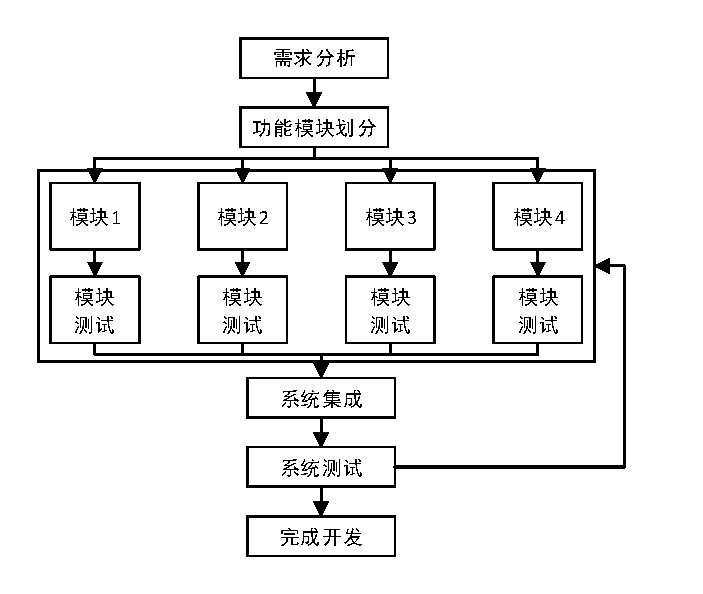
\includegraphics{../pdf/tradition.pdf}\\
        \caption{传统开发流程图}
        \label{tra}
    \end{figure}
    \begin{figure}[h]
        \centering
        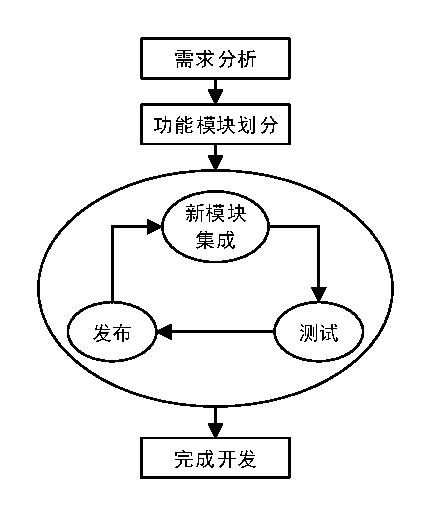
\includegraphics{../pdf/agile.pdf}\\
        \caption{敏捷型开发流程图}
        \label{agi}
    \end{figure}
    传统的开发流程可以参考图\ref{tra},可以发现开发流程呈线性,当前阶段完成后只需关注后续阶段,但用户只有等到整个过程末期才能见到开发效果,增加了开发风险,同时灵活性较低。
    敏捷型开发流程可以参考图\ref{agi},其主要开发过程呈现环状,当发布第一版之后便可见到项目雏形,同时具有高适应性可以随着开发深入遇见的问题随时调整方向。

\section{基于行静止思想的卷积计算方法}
如本章第二节所述,计划采用CPU+FPGA实现卷积神经网络的计算加速。
\begin{figure}[h]
    \centering
    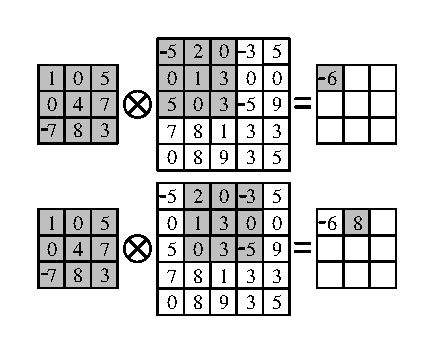
\includegraphics{../pdf/tra_conv.pdf}\\
    \caption{图像卷积计算流程}
    \label{tra_conv}
\end{figure}
传统图像卷积计算流程如图\ref{tra_conv} 所示,卷积核先与图像第一行第一列开始的同等大小矩阵进行点乘运算,计算结果进行累加得到结果的第一个值,然后卷积核在图像上向右进行滑动,再次进行点乘累加运算即可得到第二个值。
通过滑动卷积核,即可得到整张图片的卷积结果。
\begin{figure}[h]
    \centering
    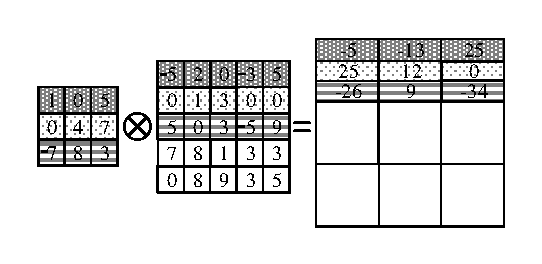
\includegraphics{../pdf/row_conv.pdf}\\
    \caption{行静止卷积计算流程}
    \label{row_conv}
\end{figure}
基于行静止思想的卷积的计算模式如图\ref{row_conv} 所示,其与普通的卷积计算模式不同,首先卷积核的第一行和图像的第一行进行一维卷积操作(图中阴影背景所标出的部分),计算结果进行缓存。
之后卷积核第二行和图像的第二行进行一维卷积操作(图中斑点背景标出部分),卷积结果和上一次按位置进行累加。
最后卷积核和图像的第三行进行一维卷积计算,得到的结果再次进行按位置累加操作,即可得到最终结果的第一行。
然后卷积核的第一、二、三行分别于图像的二、三、四行进行一维卷积操作,即可得到最终结果的第二行。
通过迭代此过程即可得到完整的卷积结果。

这种计算模式虽然不能减少计算次数,但是十分适合硬件去进行数据缓存以减少与DDR进行交互的能量消耗。



\section{本章小结}
本章首先对比传统计算架构介绍了选择异构计算的优势,其次介绍了目前主流的一些快速开发FPGA的技术,再其次引出采用Chisel3进行硬件敏捷型开发的优势及其流程,最后引出了本文所设计的加速器的核心思想。

% \subsection{二级节标题}

% \subsubsection{三级节标题}

% \paragraph{四级节标题}

% \subparagraph{五级节标题}

% \section{脚注}

% Lorem ipsum dolor sit amet, consectetur adipiscing elit, sed do eiusmod tempor
% incididunt ut labore et dolore magna aliqua. Ut enim ad minim veniam, quis
% nostrud exercitation ullamco laboris nisi ut aliquip ex ea commodo consequat.
% Duis aute irure dolor in reprehenderit in voluptate velit esse cillum dolore eu
% fugiat nulla pariatur. Excepteur sint occaecat cupidatat non proident, sunt in
% culpa qui officia deserunt mollit anim id est laborum.
% \footnote{This is a long long long long long long long long long long long long
% long long long long long long long long long long footnote.}
